\documentclass[tikz]{standalone}

\colorlet{FilledSurface}{blue!20}
\colorlet{FilledSurfaceGroupOne}{blue!20}
\colorlet{FilledSurfaceGroupTwo}{red!20}
\colorlet{FilledSurfaceGroupThree}{green!20}
\colorlet{FilledSurfaceGroupFour}{magenta!20}
\colorlet{FormulaBackground}{green!10}
\colorlet{FormulaFrame}{green}

\usetikzlibrary{calc}

\begin{document}
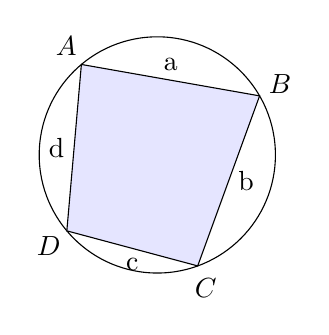
\begin{tikzpicture}

    \def\circumradius{1.5}
    \def\angleA{130}
    \def\angleB{30}
    \def\angleC{290}
    \def\angleD{220}

    \coordinate (center) at (0, 0);
    \coordinate (A) at ({\circumradius*cos(\angleA)}, {\circumradius*sin(\angleA)});
    \coordinate (B) at ({\circumradius*cos(\angleB)}, {\circumradius*sin(\angleB)});
    \coordinate (C) at ({\circumradius*cos(\angleC)}, {\circumradius*sin(\angleC)});
    \coordinate (D) at ({\circumradius*cos(\angleD)}, {\circumradius*sin(\angleD)});

    \draw (center) circle (\circumradius);

        \draw[fill=blue!10!white]
                 (A)
              -- node [above]{a} (B)
              -- node [right]{b} (C)
              -- node [below]{c} (D)
              -- node [left]{d} cycle;

    % Nombrar vértices
    \def\offset{0.3}
    \draw ($(center) + (\angleA:\circumradius + \offset)$) node {$A$};
    \draw ($(center) + (\angleB:\circumradius + \offset)$) node {$B$};
    \draw ($(center) + (\angleC:\circumradius + \offset)$) node {$C$};
    \draw ($(center) + (\angleD:\circumradius + \offset)$) node {$D$};

\end{tikzpicture}
\end{document}
